
% ----------------------------------------------------------------------------------------------------
\section{Introduction}

\begin{figure}[t]
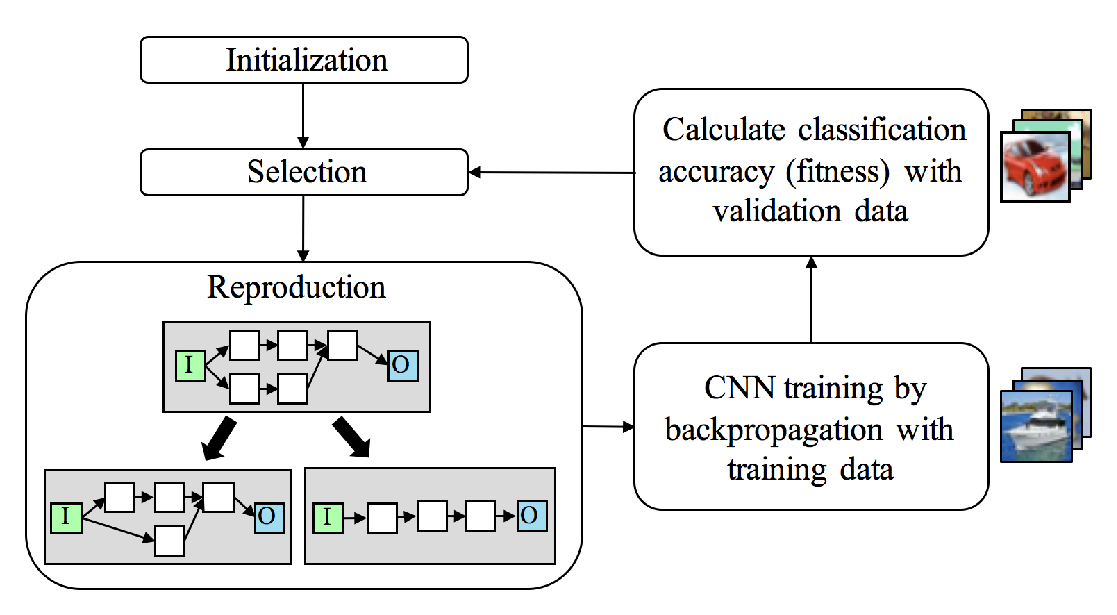
\includegraphics[scale=0.45]{images/overview.eps}
\caption{Overview of our method. Our method searches a CNN architecture using genetic programming. That CNN architecture is then trained on a learning task, and returns an accuracy. The network search is performed to maximize the accuracy by the evolutionary algorithm.}
\label{overview}
\end{figure}

Deep learning, which uses deep neural networks as a model, has shown a good performance on many challenging artificial intelligence and machine learning tasks such as image recognition \cite{lecun_gradient-based_1998,krizhevsky_imagenet_2012}, speech recognition \cite{hinton_deep_2012}, and reinforcement learning tasks \cite{mnih_playing_2013,mnih_human-level_2015}.
In particular, convolutional neural networks (CNNs) \cite{lecun_gradient-based_1998} have seen huge success in image recognition tasks in the last few years and is applied to various computer vision application, e.g. GAN \cite{goodfellow_generative_2014}, colorization \cite{zhang_colorful_2016}, image to text anotation \cite{vinyals_show_2015}.
A commonly used CNN architecture mainly consists of several convolutions, pooling, and fully connected layers.
Several recent studies focus on developing the novel CNN architecture that achieves higher classification accuracy, e. g., GoogleNet \cite{szegedy_going_2015}, ResNet \cite{he_deep_2016}, and DensNet \cite{huang_densely_2016}.
Despite their success, designing CNN architectures is still a difficult task since there exist many design parameters such as the depth of a network, the type and parameters of each layer, and the connectivity of the layers.
The state-of-the-art CNN architectures have become deep and complex, which suggests that a significant number of design parameters should be tuned to realize the best performance for a specific dataset.
Therefore, the trial and error or expert knowledge are required when the users construct the suitable architecture for their target dataset.
Because of this situation, the automatic design methods for the CNN architectures is highly beneficial.

The neural network architecture design can be viewed as the model selection problem in the machine learning. The straight-forward approach is to deal with the architecture design as the hyperparameter optimization problem, optimizing the hyperparameters such as the number of layers and neurons using black-box optimization techniques \todo{\cite{}.}

Evolutionary computation has been traditionally applied to design the neural network architectures \todo{ref. X. Yao's review, Kitano, etc...}.
There are two types of encoding schemes for the network representation: direct and indirect coding.
The direct coding represents the number and connectivity of neurons directly as the genotype, whereas the indirect coding represents a generation rule of the network architectures.
While almost traditional approaches optimize the number and connectivity of low-level neurons, the modern neural network architectures for deep learning have many units and various types of units, e.g., convolution, pooling, and normalization.
Optimizing those many parameters in reasonable computational time may be difficult.
Therefore, the use of the highly-functional modules as a minimum unit is promising.

In this paper, we attempt to design CNN architectures based on a genetic programming.
We use the Cartesian genetic programming (CGP) \cite{miller_cartesian_2000,harding_evolution_2008} encoding scheme, one of the direct encoding, to represent the CNN structure and connectivity.
The advantage of this representation is its flexibility; it can represent variable-length network structure and the skip connections.
Moreover, we adopt the relatively highly-functional modules such as convolutional blocks and tensor concatenation as the node functions in CGP to reduce the search space.
To evaluate the architecture represented by the CGP, we train the network using training dataset in an ordinary way. Then the performance for another validation dataset is assigned as the evaluation of the architecture. Based on this fitness evaluation, an evolutionary algorithm optimizes the CNN architectures.
 To check the performance of the proposed approach, we conducted the experiment constructing the CNN architecture for the image classification task with the CIFAR-10 dataset \cite{krizhevsky_learning_2009}. The experimental result shows that the proposed approach can automatically find the competitive CNN architecture compared with state-of-the-art models.

\shin{It would be nice if we can describe the research question clearly.}

The rest of this paper is organized as follows. The next section presents related work on the neural network architecture design. In Section 3, we describe our genetic programming approach to design the CNN architectures. We test the performance of the proposed approach through the experiment. Finally, in Section 5, we describe our conclusion and future work.


\begin{figure*}[t]
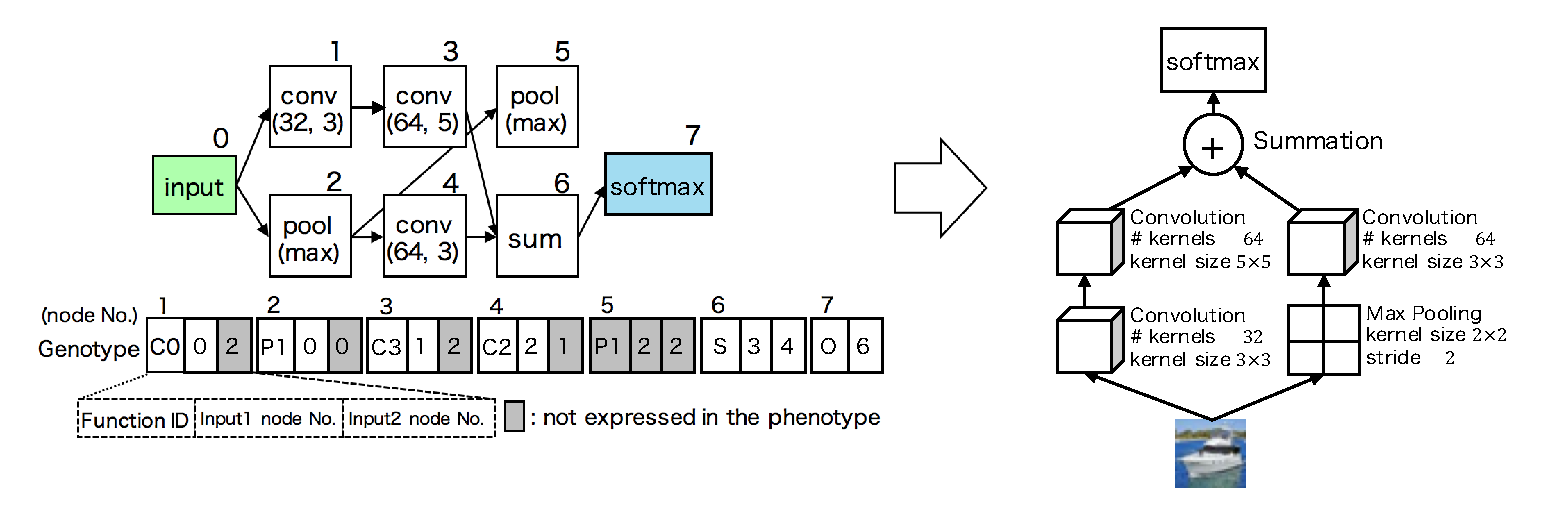
\includegraphics[scale=0.65]{images/genotype.eps}
\caption{Example of a genotype and a phenotype. The genotype (Left) defines a CNN architecture (Right).}
\label{genotype}
\end{figure*}
% ----------------------------------------------------------------------------------------------------
\section{Related Work}
%Automating neural network design and hyperparameter optimization are important topic in machine learning.
This section briefly reviews the related work on the automatic neural network architecture design: hyperparameter optimization, evolutionary neural networks, and reinforcement learning approach.

\subsection{Hyperparameter Optimization}
We can consider the neural network architecture design as the model selection or hyperparameter optimization problem from machine learning perspective. There are many hyperparameter tuning methods for the machine learning algorithm such as grid search, gradient search \cite{bengio_gradient-based_2000}, random search \cite{bergstra_random_2012}, and Bayesian optimization based methods \cite{hutter_sequential_2011,snoek_practical_2012}. Naturally, evolutionary algorithms have also been applied to the hyperparameter optimization problems \todo{\cite{} \cite{CMA etc...}.} In the machine learning community, Bayesian optimization is often used and have shown good performance in several datasets. Bayesian optimization is a global optimization method of black-box and noisy objective functions, which maintains a surrogate model learned by using previously evaluated solutions. A Gaussian process is usually adopted as the surrogate model \cite{snoek_practical_2012}, which can easily handle the uncertainty and noise of the objective function.
Bergstra et al. \cite{bergstra_algorithms_2011} have proposed the Tree-structured Parzen estimator (TPE) and shown better results than manual search and random search \cite{bergstra_random_2012}.
They have also proposed a meta-modeling approach \cite{bergstra_making_2013} based on the TPE for supporting automatic hyperparameter optimization. 
Snoek et al. \cite{snoek_scalable_2015} used a deep neural network instead of the Gaussian process to reduce the computational cost for the surrogate model building and succeeded to improve the scalability.

The hyperparameter optimization approach often tunes the predefined hyperparameters such as the number of layers and neurons, and the type of activation functions. While this method has seen success, it is hard to design more flexible architectures from scratch.

\subsection{Evolutionary Neural Networks}
Evolutionary algorithms have been used to optimize the neural network architectures so far \cite{schaffer_combinations_1992,stanley_evolving_2002}. The traditional approaches are not suitable for the model deep neural network architecture design since they usually optimize the number and connectivity of low-level neurons.

Recently, Fernando et al. \cite{fernando_convolution_2016} have proposed the differentiable pattern-producing networks (DPPNs) to optimize weights of a denoising autoencoder. The DPPN is a differentiable version of the compositional pattern-producing networks (CPPNs) \cite{stanley_compositional_2007}. This method focuses on the effectiveness of the indirect coding for weight optimization. That is, the general structure of network should be predefined.

Verbancsics et al. \cite{verbancsics_generative_2013,verbancsics_image_2015} have designed the artificial neural networks and CNN architectures with the hypercube-based neuroevolution of augmenting topologies (HyperNEAT) \cite{stanley_hypercube-based_2009}.
However, to the best of our knowledge, these networks designed with HyperNEAT have failed to match the performance of state-of-the-art methods \shin{I do not know the contents of Verbancsics's papers}.
Also, these methods deal with the architectures defined by human experts. Thus it is hard to design neural network architectures from scratch.

\subsection{Reinforcement Learning Approach}
The interesting approaches, automatic designing the deep neural network architecture using reinforcement learning, have been attempted recently \cite{zoph_neural_2016,baker_designing_2016}.
These studies showed that a reinforcement learning based method could construct the competitive CNN architectures for image classification tasks.
In \cite{zoph_neural_2016}, a recurrent neural network (RNN) is used to generate the neural network architectures, and the RNN is trained with reinforcement learning to maximize the expected accuracy on a learning task.
This method uses distributed training and asynchronous parameter updates with $800$ GPUs to accelerate the reinforcement learning process.
Baker et al. \cite{baker_designing_2016} have proposed a meta-modeling approach based on reinforcement learning to produce the CNN architectures.
A Q-learning agent explores and exploits a space of model architectures with an $\epsilon -$greedy strategy and experience replay.

These approaches adopt the indirect coding scheme for the network representation, which optimizes generative rules for the network architectures such as the RNN.
Unlike these approaches, our approach uses the direct coding based on Cartesian genetic programming to design the CNN architectures.
Besides, we introduce the relatively highly-functional modules such as convolutional blocks and tensor concatenations to find better CNN architectures efficiently.


% ----------------------------------------------------------------------------------------------------
\section{CNN Architecture Design Using Cartesian Genetic Programming}
\new{Our method directly encodes the CNN architectures based on CGP and uses the highly-functional modules as the node functions.
The CNN architecture defined by the CGP is trained using training dataset, followed by the validation accuracy is assigned as the fitness of the architecture. Then the architecture is optimized to maximize the validation accuracy by the evolutionary algorithm.

In this section, we describe the network representation, the node functions, and the evolutionary algorithm used in the proposed method.}

\shin{Checked up to here.}

\subsection{Representation of CNN Architectures}
We use a feedforward network that consists of $R$ rows by $C$ columns, i.e., the number of intermediate nodes of the network is $R\times C$.
Figure \ref{genotype} shows an example of the network of two rows by three columns and its genotype and phenotype.

The CGP inter-connectivity is determined by the levels back parameter $l$, which decides nodes of how many previous columns to connect to nodes in the current column, i.e., each node can have one or two connections to nodes in the $l$ previous columns.
Note that nodes in the same column are prohibited to be connected to each other.
The types and connections of nodes are optimized by the evolutionary algorithm.

\subsection{Node Functions}
A type of each node is represented as four different types of layers: convolution, pooling, summation, and concatenation.
The detailed parameters for each layer are shown in Table \ref{layer_param}.
The convolution node consists of a standard convolution processing with batch normalization \cite{ioffe_batch_2015} and rectified linear units \cite{nair_rectified_2010}.
The pooling node consists of the standard max pooling and average pooling processing.
The summation node performs element-wise addition of two feature maps, channel by channel. 
If input feature maps to be added have different sizes, we pad the small feature map with zeros for increasing dimensions.
The concatenation node concatenates two feature maps in the depth dimensions.
If input feature maps to be concatenated are different sizes, we pad the small feature map with zeros.
Adding these summation and concatenation nodes to the network architecture allow our method to generate shortcut connections or branching layers such as GoogleNet \cite{szegedy_going_2015} and Residual Net \cite{he_deep_2016}.

\begin{table}[tb]
  \caption{Parameter details for each layer}
  \label{layer_param}
  \begin{tabular}{l|l|l} \hline
    Node type & Parameters & Values or description \\ \hline
    Convolution & Receptive field size & $\in \{3\times 3, 5\times 5\}$ \\ 
                        & \# kernels & $\in \{32, 64, 128\}$ \\ 
                       & Stride & $1$ \\ 
                       & \# inputs & $1$ \\ \hline
      Pooling     & Receptive field size & $2\times 2$ \\ 
                       & Stride & $2$ \\ 
                       & \# inputs & $1$ \\ \hline
     Summation & \# inputs & $2$ \\ 
                         &                & Element-wise addition. \\ \hline
 Concatenation & \# inputs & $2$ \\ 
                      &  & Concatenate in the \\
                       &  & depth dimension.\\  \hline
  \end{tabular}
\end{table}


\subsection{Evolutionary Algorithm}
We use mutation as a genetic operator.
The mutation operator is applied to one individual as follows:
\begin{itemize}
  \item Select several nodes with probability $\epsilon$ for each node.
  \item Change the type and connectivity of the selected nodes randomly.
\end{itemize}
Note that we apply the mutation operator to nodes until one or more active nodes that are associated with the output path are changed.
As training a CNN can take hours, we apply the above mutation operator to save time.

We use a simple form of $(1+\lambda)$ evolutionary strategy (with $\lambda = 2$) to design CNN architectures.
The algorithm is as follows:
\begin{description}
  \item[1.] Generate an initial individual at random as a parent $M$, and train the CNN defined by $M$.
  \item[2.] Generate a set of two offsprings $C$ by applying the mutation operation to $M$.
  \item[3.] Train these two CNNs defined by offsprings $C$.
  \item[4.] Select an elite individual from the set of $M$ and $C$, and replace $M$ with the elite individual.
  \item[5.] Return to step $2$ until a stopping criterion is satisfied.
\end{description}
We employ the accuracy of the CNN on a validation set as the fitness of each individual.


% ----------------------------------------------------------------------------------------------------
\section{Experiments and Results}
\subsection{Dataset}
We test our method to the image classification task with CIFAR-10 dataset which has $10$ classes with $50,000$ training images and $10,000$ test images.
We sampled $5,000$ images randomly from the training set for the validation set, the remaining $45,000$ images are used as the training set.
In this experiment, we use data preprocessing and augmentation procedure.
We first preprocess the data with the per-pixel mean subtraction.
We then pad $4$ pixels on each side, and choose a random $32\times 32$ crop from the padded image.
At last, we perform random horizontal flips on the cropped $32 \times 32$ image. 

\subsection{Training details}

\begin{table}[t]
  \caption{Parameter settings for the CGP}
  \label{cgp_param}
  \begin{tabular}{l|l} \hline
    Parameters & Values or description \\ \hline
   \# generations & $300$ \\ 
   Mutation rate & $0.05$ \\
   \#  rows & $5$ \\
   \#  columns & $30$ \\
   Levels back & $10$ \\
   Generation alternation model & $(1+2)$ Evolution Strategy \\ \hline
  \end{tabular}
\end{table}

Parameter settings for the CGP is shown in Table \ref{cgp_param}.
Once the CGP samples a CNN architecture, every CNN is trained for $50$ epochs with the Adam optimizer \cite{kingma_adam:_2015} with an initial learning rate of $0.01$.
We reduce the learning rate by a factor of $10$ every $20$ epochs.
All weights of CNN are initialized with He \cite{he_delving_2015}, and the mini-batch size is set to $128$.

After finishing the evolution of the CGP, we select the architecture that showed the best validation accuracy.
We then fine-tune the best model with a different training schedule.
During this phase, we set a learning rate to $0.01$ for $50$ epochs, then $0.001$ for $50$ epochs.
The other parameters are unchanged.
After training the best model, we apply the model to the test set.

\subsection{Results}

\begin{table}[t]
  \caption{Comparison of error rate on CIFAR-10 dataset.}
  \label{results}
  \begin{tabular}{l|c|c} \hline
    Model & Error rate & \# params ($10^6$) \\ \hline
   Maxout \cite{} & $9.38$ & - \\ 
   MetaQNN \cite{baker_designing_2016} \footnotemark & $9.09$ & $3.7$ \\
   Network in Network \cite{} & $8.81$ & - \\
   CGP2CNN (A) & $8.17$ & $1.58$ \\
   VGG \cite{simonyan_very_2014} \footnotemark & $7.94$ & $15.2$ \\
   CGP2CNN (B) & $7.74$ & $1.68$ \\
   ResNet \cite{he_deep_2016} & $6.61$ & $1.7$ \\
   Neural Architecture Search \cite{zoph_neural_2016} & $3.84$ & $32.0$ \\ \hline
   %\multicolumn{1}{l}{*The mean error rate and the number of parameters of top $5$ models.} & \multicolumn{1}{l}{} & \multicolumn{1}{l}{} \\
  \end{tabular}
\end{table}
\footnotetext[1]{The mean error rate and the number of parameters of top $5$ models are shown.}
\footnotetext{We implemented the VGG net \cite{simonyan_very_2014} and applied the model to the CIFAR-10 dataset since the 
VGG net is not applied to the CIFAR-10 dataset in \cite{simonyan_very_2014}.
The architecture of the VGG is identical with the configuration D in \cite{simonyan_very_2014}.
We denote this model as VGG in this paper.}

We compare the classification performance of our method with the state-of-the-art-methods and summarize the results in Table \ref{results}.
We refer to our architecture designed using functions in Table \ref{layer_param} as CGP2CNN (A) and the architecture designed using ResBlock as CGP2CNN (B).
As can be seen in Table \ref{results}, our method can design architectures that are competitive with the state-of-the-art-methods.
In addition, our architectures have a good balance between classification accuracy and the number of parameters.
In this experiment, CGP2CNN (B) shows a better performance than that of CGP2CNN (A).
The architecture of CGP2CNN (B) is shown in Figure \ref{model}.
A notable feature of this architecture is that it has a similar structure to the ResNet \cite{he_deep_2016}.
The architecture of the ResNet \cite{he_deep_2016} has the pairs of $3\times 3$ convolution layers and convolution layers that performs downsampling by convolution that have a stride of $2$.
Although our method cannot perform downsampling by convolution layers, we can see from Figure \ref{model} that CGP2CNN (B) uses average pooling as an alternative to the convolution layers for downsampling.
Also, CGP2CNN (B) has the pairs of $3\times 3$ convolution layers similar to the ResNet.
It follows from what has been said that our method can design a architecture similar to one designed by experts.
\suga{the rest of sentence is depending on experiment results...}


\begin{figure}[!t]
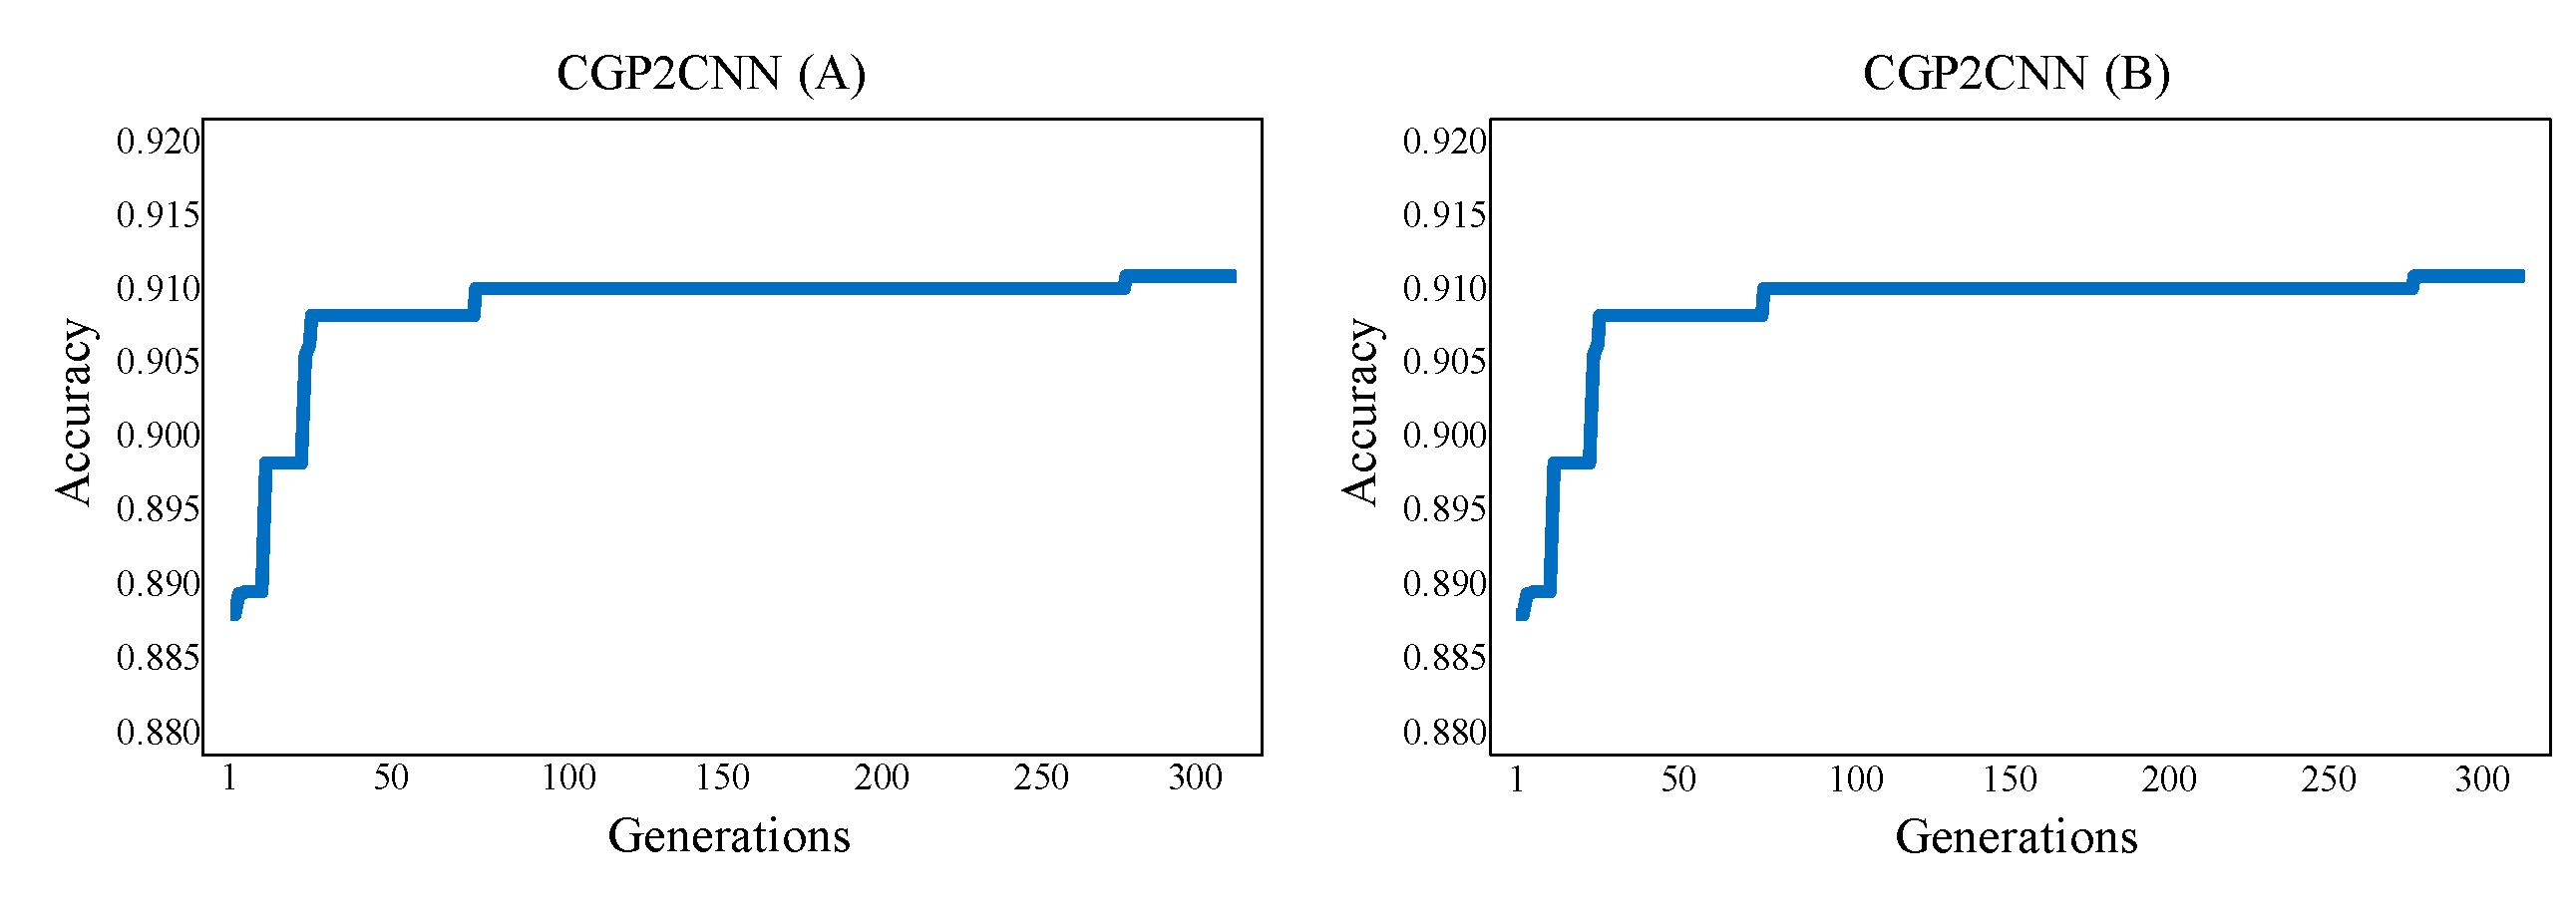
\includegraphics[scale=0.4]{images/fitness.eps}
\caption{Transition of the fitness of CGP2CNN (A).}
\label{fitness}
\end{figure}

\begin{figure}[t]
\includegraphics[scale=0.5]{images/model.eps}
\caption{CNN architecture designed by our method. $ResBlock(n, k)$ denotes a ResBlock node with $n$ filters and receptive field size $k$.}
\label{model}
\end{figure}


\subsection{Designing architectures with a small dataset}

\begin{table}[t]
  \caption{Comparison of error rate with the small CIFAR-10 dataset.}
  \label{results_small}
  \begin{tabular}{l|c} \hline
    Model & Error rate \\ \hline
   VGG \cite{simonyan_very_2014} & $27.67$ \\
   ResNet \cite{he_deep_2016} & $24.10$ \\ 
   CGP2CNN (A) & $22.82$  \\
   CGP2CNN (B) & $-$ \\ \hline
  \end{tabular}
\end{table}


To test the robustness of our method, we design a architecture with a small CIFAR-10 dataset that consists of $5,000$ images randomly chosen from the CIFAR-10 dataset. 
We sampled $500$ images randomly from the small training set for the validation set, the remaining $4,500$ images are used as the training set.
For settings of our method, the number of generation is set to $2,000$.
The other experimental settings are the same in the preceding section.
We compare our method with the VGG and ResNet.
For the VGG settings, the VGG is trained for $200$ epochs with SGD with an initial learning rate of $0.01$.
We reduce the learning rate by a factor of $10$ every $50$ epochs.
The mini-batch size is set to $128$.
For the ResNet, we train the model for $500$ epochs.
We use SGD with the mini-batch size of $128$.
We start with a learning rate of $0.1$, then divide it by $10$ at $250$ and $375$ epochs.

Table \ref{results_small} shows that even with a small dataset, our model can find better architectures than the VGG and ResNet.
The best architecture is shown Figure \ref{model_small}.
\suga{the rest of sentence is depending on experiment results...}

\section{Conclusions}


